\documentclass[conference]{IEEEtran}
\usepackage[T1]{fontenc}
\usepackage{tgtermes}
\usepackage{cite}
\usepackage{amsmath}
\usepackage{graphicx}
\usepackage{booktabs}
\usepackage{array}
\usepackage{url}
\graphicspath{{../figures/}}
% Generated from held-out prediction summaries.
\newcommand{\SentinelCount}{277}
\newcommand{\AnyCount}{331}
\newcommand{\MisaRmse}{1.763}
\newcommand{\MisaMae}{1.237}
\newcommand{\MisaRsq}{0.325}
\newcommand{\DeltaVone}{\ensuremath{-0.079}}
\newcommand{\DeltaVoneCI}{\mbox{$[-0.146,\,-0.017]$}}
\newcommand{\AbstractVerdict}{ExtraTrees without Landsat scored RMSE 1.729 \unit{}. Overall superiority of MISA was unsupported.}
\newcommand{\ConclusionText}{Optical coverage improved, but the matched evaluation did not establish overall superiority for the missingness-informed ensemble.}
\newcommand{\CoverageText}{Landsat matched 325 sites and recovered optical predictors at 54 of the 72 originally unmatched sites. Among the 38 high-EC sites, availability changed from 14 to 30. Local terrain derivatives were available for 348 sites.}
\newcommand{\PriorFailureText}{Mean EC was 4.226 \unit{} without Sentinel-2 and 1.499 \unit{} with Sentinel-2. V1 Auto spatial RMSE was 2.681 and 1.551 \unit{} in those respective groups.}
\newcommand{\SpatialText}{MISA scored 1.763 \unit{} RMSE, 1.237 \unit{} MAE and $R^2=0.325$. Its RMSE difference against V1 Auto was \ensuremath{-0.079} \unit{} (\mbox{$[-0.146,\,-0.017]$}), a +4.3\% relative reduction.}
\newcommand{\CompareText}{The lowest point estimate was 1.729 \unit{} for ExtraTrees without Landsat. Against ExtraTrees without Landsat, the MISA difference was \ensuremath{+0.033} \unit{} (\mbox{$[-0.051,\,0.095]$}).}
\newcommand{\SubgroupText}{For EC at or above 5 \unit{}, MISA MAE was 3.643 \unit{} and bias was \ensuremath{-3.643} \unit{}, compared with 3.780 and \ensuremath{-3.780} \unit{} for V1 Auto. The paired high-EC MAE difference was \ensuremath{-0.137} \unit{} (\mbox{$[-0.416,\,0.370]$}). Without Sentinel-2, the paired MAE difference against V1 Auto was \ensuremath{-0.052} \unit{} (\mbox{$[-0.367,\,0.112]$}).}
\newcommand{\TransferText}{Transfer RMSE was 2.377 \unit{} ($R^2=0.070$) for 2024 to 2025 and 1.529 \unit{} ($R^2=0.007$) in reverse. The buffered counterparts were 2.399 and 1.674 \unit{}.}
\newcommand{\AblationText}{Equal-budget ExtraTrees RMSE was 1.779 \unit{} with full inputs, 1.742 with V1 inputs and 1.772 without availability flags. Log targets yielded 1.788 and high-EC weighting 1.824 \unit{}. The same MISA experts gave 1.773 with global and 1.792 with equal weights. Removing Landsat gave 1.729 \unit{}.}
\newcommand{\HighWeightText}{High-EC weighting in Huber boosting reduced high-EC MAE from 3.900 to 3.480 \unit{} (paired difference \ensuremath{-0.420}, \mbox{$[-0.625,\,-0.146]$}). The pooled RMSE increased from 1.772 to 1.845 \unit{}. Weighted random forest and extra trees showed the same trade-off.}
\newcommand{\ImportanceText}{Mean RMSE changes were \ensuremath{+0.062} for Terrain, \ensuremath{+0.061} for Sentinel-2, \ensuremath{+0.031} for Landsat, \ensuremath{+0.016} for Location \unit{}.}
\newcommand{\LeaderRows}{
V1 Auto & 349 & 1.842 & 1.312 & 0.263 & \ensuremath{+0.000} \\
V1 ExtraTrees* & 349 & 1.746 & 1.268 & 0.338 & \ensuremath{-0.096} \\
Mean & 349 & 2.245 & 1.712 & -0.095 & \ensuremath{+0.403} \\
IDW & 349 & 1.994 & 1.448 & 0.137 & \ensuremath{+0.152} \\
Ridge & 349 & 1.755 & 1.245 & 0.331 & \ensuremath{-0.087} \\
RF & 349 & 1.854 & 1.324 & 0.253 & \ensuremath{+0.012} \\
ExtraTrees & 349 & 1.771 & 1.241 & 0.318 & \ensuremath{-0.071} \\
SVR & 349 & 1.814 & 1.184 & 0.285 & \ensuremath{-0.028} \\
XGBoost & 349 & 1.915 & 1.385 & 0.203 & \ensuremath{+0.073} \\
LightGBM & 349 & 1.910 & 1.353 & 0.207 & \ensuremath{+0.068} \\
CatBoost & 349 & 1.784 & 1.275 & 0.308 & \ensuremath{-0.058} \\
AdaBoost & 349 & 1.856 & 1.394 & 0.252 & \ensuremath{+0.014} \\
Huber-GB & 349 & 1.761 & 1.216 & 0.326 & \ensuremath{-0.081} \\
XGB + spline & 349 & 1.953 & 1.358 & 0.171 & \ensuremath{+0.111} \\
Inner winner & 349 & 1.787 & 1.298 & 0.306 & \ensuremath{-0.055} \\
MISA & 349 & 1.763 & 1.237 & 0.325 & \ensuremath{-0.079} \\
MISA global & 349 & 1.773 & 1.254 & 0.317 & \ensuremath{-0.070} \\
MISA equal & 349 & 1.792 & 1.264 & 0.302 & \ensuremath{-0.050} \\
ExtraTrees without Landsat & 349 & \textbf{1.729} & 1.244 & 0.350 & \ensuremath{-0.113} \\
}

\newcommand{\EC}{\ensuremath{\mathrm{EC}_{1:5}}}
\newcommand{\unit}{\ensuremath{\mathrm{mS\,cm^{-1}}}}
\newcolumntype{P}[1]{>{\raggedright\arraybackslash}p{#1}}
\begin{document}

\title{Benchmarking Machine Learning for Multi-Year Soil Salinity Prediction in Coastal Bangladesh: Spatial and Temporal Generalization}
\author{\IEEEauthorblockN{Kamrunnahar Rima and Sheikh Hasiba}
\IEEEauthorblockA{Department of Computer Science and Engineering\\
Bangladesh University, Dhaka, Bangladesh}}
\maketitle

\begin{abstract}
Soil salinity prediction requires evidence that models transfer to new locations and field campaigns. We reanalyzed 349 publicly archived topsoil measurements of electrical conductivity in a 1:5 soil--water extract from coastal southwestern Bangladesh, using 162 records from March 2024 and 187 from April 2025. We compared spatial interpolation and regression baselines with models using pre-collection Sentinel-2 surface reflectance and Copernicus surface elevation. Model selection used buffered inner spatial folds, with six buffered spatial test folds and two independent campaign transfers. The prespecified all-predictor selection procedure achieved pooled spatial RMSE of \SpatialRMSE{} \unit{} ($R^2=\SpatialRsq$) and campaign-transfer RMSE of \ForwardRMSE{} and \ReverseRMSE{} \unit{}, respectively. In spatial cross-validation, its paired RMSE difference versus tuned inverse distance weighting was \SpatialDelta{} \unit{} (95\% spatial-block bootstrap interval \SpatialDeltaCI). The published Satkhira benchmark uses different evaluation records and Landsat predictors, so these results quantify performance on our protocol. The two campaigns differ in both location and sampling month, which limits interpretation of transfer errors as interannual change.
\end{abstract}
\begin{IEEEkeywords}
soil electrical conductivity, Sentinel-2, spatial cross-validation, domain shift, Bangladesh
\end{IEEEkeywords}

\section{Introduction}
Field measurements provide an empirical basis for mapping soil salinity in coastal Bangladesh \cite{descriptor}. At unmeasured locations, however, a predictor may benefit from geographic proximity to known samples, or from environmental covariates that are informative outside the sampled region. A model can also learn relationships that change when sampling shifts to a new month or a different set of sites. These are distinct prediction problems. An evaluation that randomly separates observations can retain nearby sites on both sides of the split and estimate a different task from geographic extrapolation \cite{roberts}.

We benchmark point prediction of \EC{} on the full public releases from two campaigns \cite{data24,data25}. We evaluate geographic and bidirectional campaign holdouts, optical and elevation enrichment, feature selection, and model tuning. We archive the per-site imagery cutoffs, split distances, and held-out predictions. Sarkar and Ravela already combine these data sources with remote sensing, spatial CV, and uncertainty assessment for Satkhira \cite{dynamic}.

\section{Related Work}
The interpolation study on the 2024 samples \cite{rootzone} motivates our inverse distance weighting (IDW) comparator. The other studies in Table~\ref{tab:related} differ in sampling, target or predictors. ROC AUC measures discrimination \cite{coupling}, Jia et al.\ predict converted salt concentration \cite{jia}, and Arshad et al.\ use additional laboratory covariates \cite{arshad}.

\begin{table*}[!t]
\caption{Primary-source benchmarks and their limits for this study. Performance is quoted on the authors' evaluation protocols.}
\label{tab:related}
\centering
\small
\begin{tabular}{@{}P{.15\textwidth}P{.22\textwidth}P{.25\textwidth}P{.30\textwidth}@{}}
\toprule
Author & Method & Accuracy/Performance & Limitations \\
\midrule
Sarkar and Ravela (2026) \cite{dynamic} &
Landsat 8 indices; XGBoost; spline GAM for mapping; six geographic folds &
2024: $R^2=0.912$, RMSE $=0.454$ \unit. 2025: $R^2=0.856$, RMSE $=0.997$ \unit. &
Preprint. Satkhira subset (86 and 119 records) from the two workbooks. Identical row and fold keys are unavailable. \\
Sarkar et al.\ (2024) \cite{rootzone} &
Spatial interpolation, including empirical Bayesian kriging &
Best reported leave-one-out RMSE $=1.3$ \unit. &
Preprint. Same 162 records for 2024. Leave-one-out permits nearby training sites. \\
Sarkar et al.\ (2023) \cite{coupling} &
Landsat indices; random forest, bagged random forest, neural network &
ANN ROC AUC $=0.921$. &
241 earlier Satkhira records and an 80/20 allocation. Classification AUC and EC regression errors quantify different outcomes. \\
Jia et al.\ (2024) \cite{jia} &
Sentinel-2 and environmental covariates; feature screening and regression &
Best coastal AdaBoost after GBM screening: $R^2=0.77$, RMSE $=1.74$ g/kg. &
98 coastal and 231 arid samples in China. Target is derived salt mass concentration. The paper reports 10-fold CV. \\
Arshad et al.\ (2025) \cite{arshad} &
Sentinel-1/2, topography and laboratory soil attributes; improved FFNN/LSTM ensemble &
Test $R^2=0.841$, RMSE $=1.382$, MAE $=1.014$ dS/m. &
109 samples in Pakistan; 28 test samples from a random split. Additional laboratory inputs and an annual optical composite. \\
\bottomrule
\end{tabular}
\end{table*}

\subsection{The Satkhira benchmark}
The 2026 preprint uses 13 predictors at 30 m from Landsat 8 Collection 2 Tier 1 Level-2 imagery, WRS-2 path 138 and row 44, and an annual February--April window \cite[Sec.~2.3]{dynamic}. Its stated window can extend past sampling. The authors use six coordinate $k$-means groups, seed 123 and 50 starts, and tune XGBoost in a grid with spatial resampling. They fit the mapping GAM on out-of-fold XGBoost predictions. The description does not establish a separate outer evaluation of the tuning and calibration procedure or state whether the scatterplot metrics include calibration. We therefore quote those results as the preprint's reported spatial CV scores.

We independently intersected workbook coordinates with a pinned public Satkhira district polygon \cite{geoboundaries}. It yielded \BoundaryCount{} candidate records. Polygon membership is an approximation to the authors' sampling and complete-predictor rules. Exact comparison requires the author's row-level subset, input rasters or feature matrix, fold membership, and the implementation used to generate the reported predictions. Our six folds use a different region, a buffer, and a nested search. We leave direct replication unresolved and make no claim of exceeding the published baseline.

\section{Data and Study Area}
The field data were collected and assayed by the Zenodo creators \cite{data24,data25}. This study is a secondary computational analysis. The 2024 descriptor describes composite sampling from approximately $30\times30$ m plots and excavation to 30 cm \cite{descriptor}. Both campaigns used a 1:5 soil--water extraction and a Hanna HI-6321 meter \cite{descriptor,data25}. We retain the workbook unit of \unit. The extract differs from a saturated paste. We neither convert to saturated-paste conductivity nor assign salinity classes.

The worksheets contain laboratory metadata above row 3 and a copyright footer after the measurements. We verified the published file hashes, recorded every field row, and retained all 349 observations with finite nonnegative EC, valid regional coordinates and soil sample type. Coordinates were used as supplied in geographic degrees and projected to WGS84/UTM zone 45N for distances. There are no exact duplicate coordinates. One same-year pair is within 20 m, and the median distance to the other campaign's nearest site is 3.07 km from 2024 and 2.98 km from 2025.

\begin{figure*}[!t]
\centering
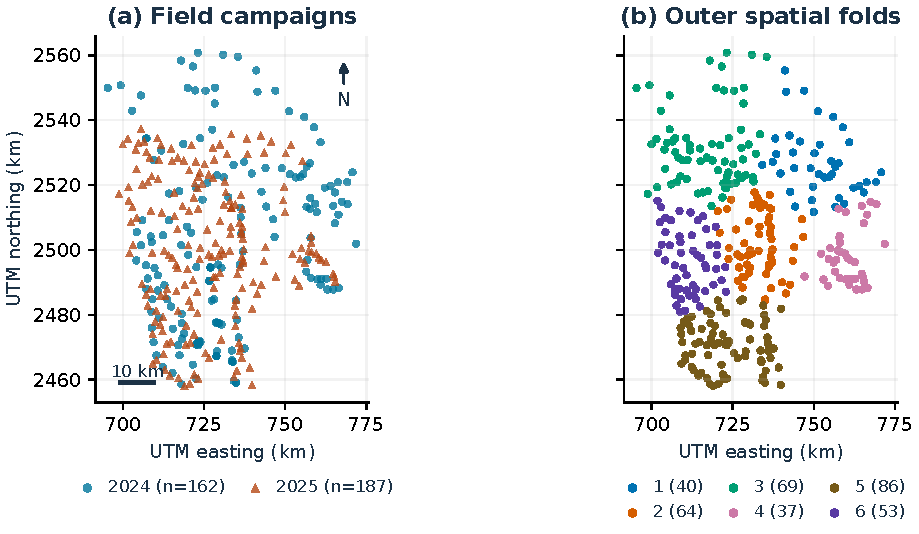
\includegraphics[width=.96\textwidth]{study_area}
\caption{Field records projected to WGS84/UTM zone 45N. (a) Campaign locations and grid north. (b) Six outer $k$-means holdout clusters, with fold number and sample count. Training observations within 1 km of a held-out point are excluded per fold.}
\label{fig:map}
\end{figure*}

Figure~\ref{fig:map} shows that the 2024 campaign extended farther north. The descriptor gives a wider March campaign window \cite{descriptor}, whereas the actual date cells span 2--6 March. The 2025 cells span 11--14 April. Median observed EC is 1.14 in 2024 and 1.748 \unit{} in 2025. The observed maxima are 9.085 and 10.50 \unit{}. Figure~\ref{fig:ec} gives the empirical cumulative distributions. Different observation locations and sampling months preclude estimating site-level change from these distributions.

\begin{figure}[t]
\centering
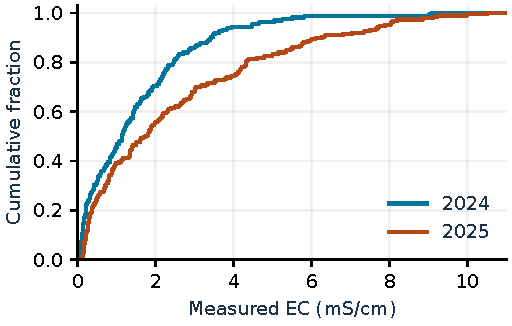
\includegraphics[width=\columnwidth]{ec_distribution}
\caption{Empirical distributions of measured 1:5 EC for the two complete campaigns.}
\label{fig:ec}
\end{figure}

\section{Methodology}
\subsection{Predictors available before collection}
For each sample we search the Earth Search archive for Sentinel-2 Collection-1 L2A scenes acquired 1--30 days before the local collection date \cite{earthsearch,sentinel}. Same-day scenes are excluded because field timestamps are unavailable. We sample the containing native pixel at each point, using the newest eligible scene with a vegetation or bare-soil scene classification (SCL 4 or 5) and all six valid band values. This excludes water, cloud, shadow, snow and other uncertain classifications. We use the asset-specific reflectance transform $\rho=s\,\mathrm{DN}+o$ and retain source scene and lag. We sample B02, B03, B04 and B08 at 10 m and B11 and B12 at 20 m. Optical availability and the lag distribution are reported in Sec.~\ref{sec:results}.

We compute NDVI and NDMI as $(\rho_\mathrm{NIR}-\rho_b)/(\rho_\mathrm{NIR}+\rho_b)$ with $b$ equal to red and SWIR1, respectively \cite{ndvi,ndmi}. A denominator at or below $10^{-6}$ yields a missing index and valid ratios are clipped to $[-1,1]$. These covariates can capture canopy and moisture variation. The Copernicus GLO-30 DSM is a static, pre-campaign surface elevation covariate \cite{dem}. Height includes vegetation and structures where present. Collection dates are used for satellite alignment and transfer partitions only. Neither year nor source metadata enter any predictor set.

\begin{table}[t]
\caption{Predefined predictor groups. Auto selects a family and hyperparameters within each group.}
\label{tab:features}
\centering
\small
\begin{tabular}{@{}lp{.81\columnwidth}@{}}
\toprule
Set & Predictors \\
\midrule
A & UTM coordinates (geographic baseline) \\
B & Six reflectance bands, NDVI and NDMI \\
C & B plus Copernicus surface elevation \\
D & Three or five training-selected predictors from C \\
E & A plus C (all predictors) \\
\bottomrule
\end{tabular}
\end{table}

\subsection{Candidate models}
The baseline ladder includes the training mean and median, ordinary least squares, ridge, elastic net, KNN, support vector regression, and IDW. For a location $\mathbf{x}$, IDW uses the $k$ nearest training locations and predicts
\begin{equation}
\widehat y(\mathbf{x}) =
  \frac{\sum_{j=1}^{k} d_j^{-p} y_j}{\sum_{j=1}^{k}d_j^{-p}},
  \qquad d_j=\|\mathbf{x}-\mathbf{x}_j\|_2 .
\end{equation}
Exact coordinate matches, if present, use the mean of their responses. Ridge minimizes squared errors plus $\alpha\|\boldsymbol\beta\|_2^2$. The coordinate comparisons also include random forest, extremely randomized trees, gradient boosting, XGBoost, LightGBM and CatBoost. For Sets B--E we compare ridge, SVR and the tree-based families. A fixed random forest provides a reference for the effect of tuning within the same model family.

We impute missing predictors using training medians, retaining empty columns as constants, and scale inputs only for distance-based or linear learners other than IDW. Set D selects the three or five largest univariate training-fold regression $F$ scores. We predict in original EC units with negative outputs clipped to zero. The procedure labeled Auto chooses the family and candidate parameters with lowest pooled inner-fold RMSE for the feature set in question. It is assessed by predicting the outer fold once with that selected pipeline. Auto is a selection rule and does not combine predictions from different families.

\begin{figure*}[!t]
\centering
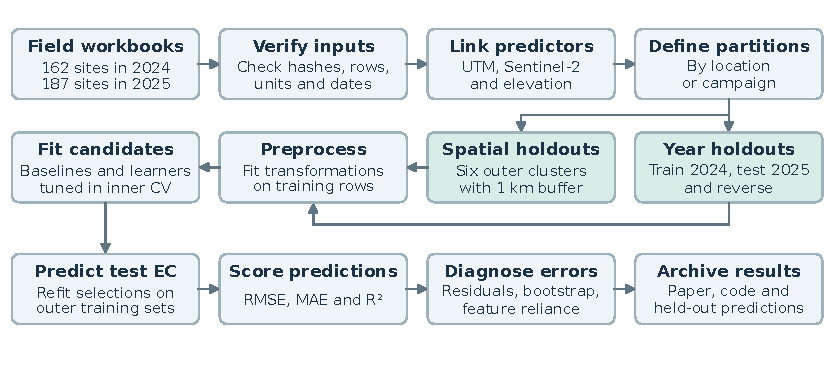
\includegraphics[width=.97\textwidth]{workflow}
\caption{Data and evaluation workflow. The spatial and campaign tracks each define their own outer test partitions before preprocessing, candidate selection, and refitting. Held-out predictions feed all error analyses.}
\label{fig:workflow}
\end{figure*}

\section{Experimental Setup and Reproducibility}
\subsection{Spatial and campaign tests}
Figure~\ref{fig:workflow} summarizes the evaluation. Track II uses six $k$-means groups of projected coordinates, independent of EC, from the pooled dataset. For each fold, the group is held out and training rows less than 1 km from any test point are removed. This prevents both sides of a spatial split sharing a near-duplicate location or native satellite pixel. The geometry is transductive in the sense that all coordinates inform the outer partition. Fitting and selection use the training data only.

Track III trains on either complete year and assesses predictions on the other complete year. In each direction the training-year data alone define the inner splits and model selection. The main campaign tests allow geographic overlap as part of operational transfer. Track IV removes training points within 1 km of any target campaign point, retaining the entire test set and redoing all tuning within the reduced training set. This sensitivity analysis changes both training size and distance.

Each outer training set is reclustered into four inner spatial groups with the same buffer rule. We use seed 123, 50 starts for $k$-means, a fixed candidate grid, and single-threaded model fitting. Each candidate is ranked by total inner squared error divided by the number of predicted rows before taking the square root. After selection, the pipeline is refit to the eligible outer training records. The archive includes split membership, inner fold scores, every candidate's parameters, runtimes, warnings, selected models and package versions. The reference run used CPython 3.14.3 on Windows 11 with an AMD Ryzen 5 5600 CPU.

\begin{table*}[!t]
\centering
\caption{Held-out RMSE and MAE in \unit{}, with dimensionless $R^2$. Rows labeled Auto are independently selected by inner-fold RMSE. Lower RMSE and MAE indicate smaller errors.}
\label{tab:results}
\small
\begin{tabular}{@{}lrrrrrrrrr@{}}
\toprule
 & \multicolumn{3}{c}{Spatial CV ($n=349$)} &
 \multicolumn{3}{c}{2024 $\rightarrow$ 2025 ($n=187$)} &
 \multicolumn{3}{c}{2025 $\rightarrow$ 2024 ($n=162$)} \\
\cmidrule(lr){2-4}\cmidrule(lr){5-7}\cmidrule(lr){8-10}
Predictors and estimator & RMSE & MAE & $R^2$ & RMSE & MAE & $R^2$ & RMSE & MAE & $R^2$ \\
\midrule
\ResultRows
\bottomrule
\end{tabular}
\end{table*}

\begin{figure*}[!t]
\centering
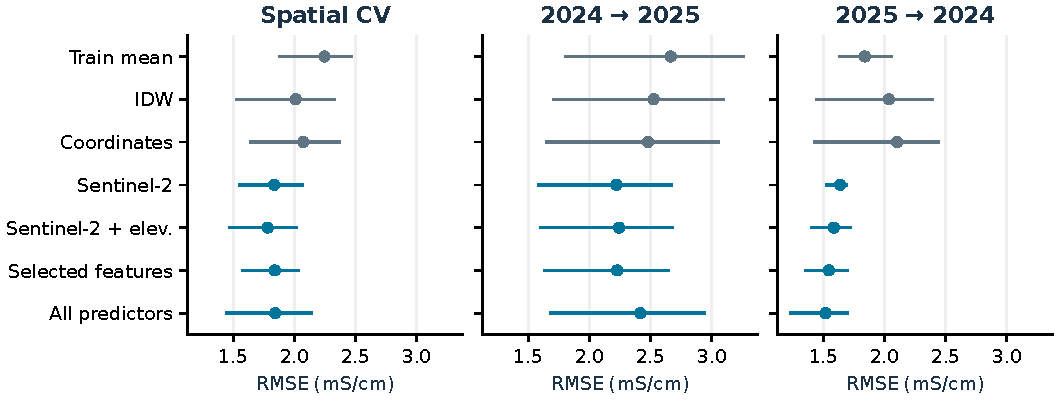
\includegraphics[width=.98\textwidth]{model_comparison}
\caption{Pooled held-out RMSE by test design. Bars are 95\% spatial-block bootstrap intervals conditional on the predictions. Feature group rows use the inner-CV Auto selection procedure.}
\label{fig:performance}
\end{figure*}

\begin{figure*}[!t]
\centering
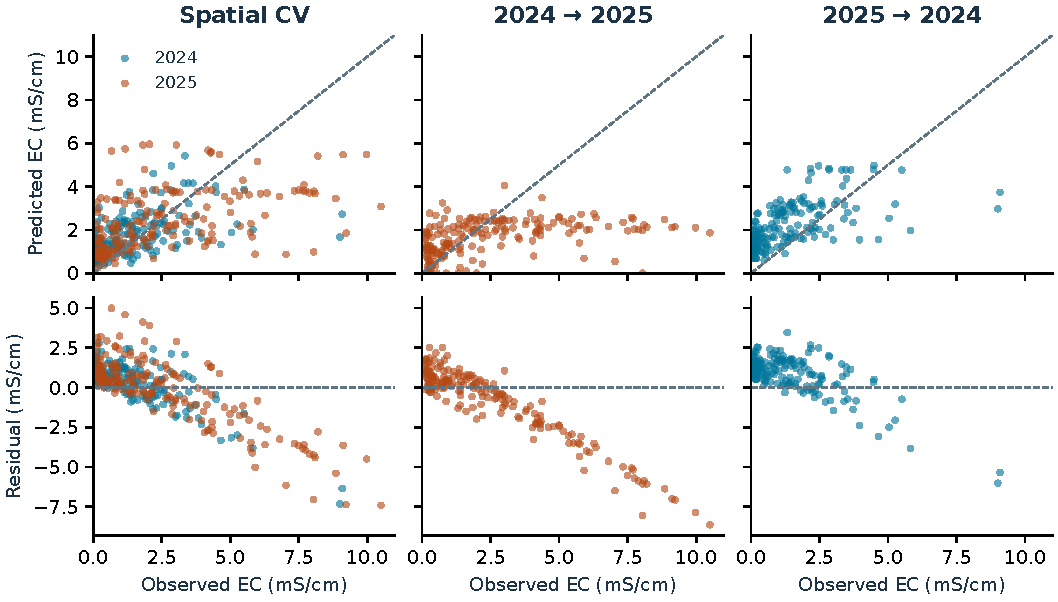
\includegraphics[width=.97\textwidth]{diagnostics}
\caption{Set E Auto predictions against observations (top) and signed residuals (bottom). All marks are held-out records. The upper diagonal is exact agreement and the lower line is zero residual.}
\label{fig:diagnostics}
\end{figure*}

\subsection{Scoring and diagnostics}
For $n$ held-out predictions and residuals $e_i=\widehat y_i-y_i$, we calculate
\begin{align}
\mathrm{RMSE}&=\sqrt{n^{-1}\sum_i e_i^2},&
\mathrm{MAE}&=n^{-1}\sum_i |e_i|,\\
R^2&=1-\frac{\sum_i e_i^2}{\sum_i(y_i-\bar y)^2},&
\mathrm{bias}&=n^{-1}\sum_i e_i .
\end{align}
The mean $\bar y$ is computed from the evaluation labels for scoring only. We pool out-of-fold predictions, so a larger fold contributes more observations. In each track we resample six intact spatial groups with replacement 4,000 times, using outer groups for Track II and coordinate groups of test sites for Track III and IV. We use identical draws for paired comparisons. The intervals describe variation across the observed spatial groups conditional on fitted predictions. They do not account for refitting uncertainty. With only six groups and overlapping training sets, coverage is uncertain.

We summarize errors by campaign, outer region and fixed EC ranges. For the all-predictor selection procedure, we also permute coordinate, optical and elevation groups jointly within each held-out fold, averaging over 20 permutations. Grouping correlated optical predictors avoids permuting a band independently of indices derived from it. Joint permutations can still break dependence between predictor groups.

\section{Results}
\label{sec:results}
\subsection{Coverage and pooled spatial performance}
\CoverageText{}
Table~\ref{tab:results} and Fig.~\ref{fig:performance} compare predictions made for the same rows within each track. In buffered spatial CV, the all-predictor procedure gave RMSE \SpatialRMSE{} \unit{}, versus \SpatialIDW{} for tuned IDW and \SpatialMean{} for the training mean. The paired difference versus IDW was \SpatialDelta{} \unit{} with interval \SpatialDeltaCI. The difference versus coordinate-only selection was \CoordDelta{} \unit{} with interval \CoordDeltaCI. \SpatialInterpretation{}

\subsection{Feature groups and tuning}
\AblationText{} \TuningText{} \SelectionText{} \DescriptiveText{} The supplementary tables give every fitted family by feature set.

\subsection{Campaign transfer and distance sensitivity}
The all-predictor selection procedure produced \ForwardRMSE{} \unit{} RMSE for 2024 to 2025 and \ReverseRMSE{} \unit{} for the reverse direction. The held-out campaigns differ in target variance and support, so lower RMSE in one direction alone cannot establish stronger transportability. \TransferText{} With a 1 km transfer buffer, we obtained \BufferedForward{} and \BufferedReverse{} \unit{}, respectively, for Set E. This sensitivity check removes 8 and 9 training records. It preserves the held-out campaign and helps distinguish dependence on nearby training locations from broader transfer failure, although the change in fitted training samples contributes to the difference.

\subsection{Residuals and predictor reliance}
Figure~\ref{fig:diagnostics} shows the relationship between predicted and measured EC. \ResidualText{} Figure~\ref{fig:residualmap} plots point errors without interpolating residuals between sites. Figure~\ref{fig:importance} reports held-out permutation error changes. \ImportanceText{} These changes reflect the model's reliance on the sampled predictors under artificial perturbations. They do not estimate soil processes or causal effects.

\begin{figure}[t]
\centering
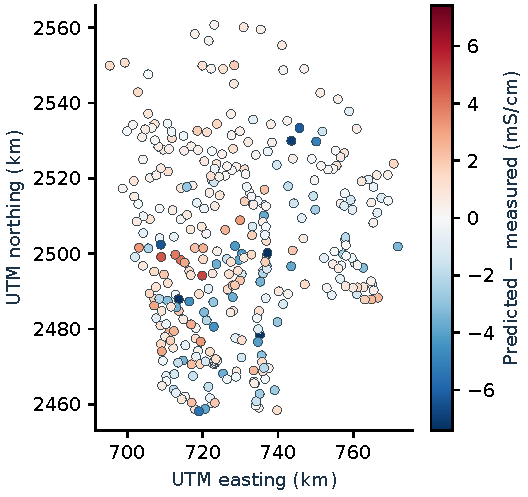
\includegraphics[width=\columnwidth]{spatial_errors}
\caption{Signed point residuals for Set E Auto in buffered spatial CV. Negative values denote underprediction.}
\label{fig:residualmap}
\end{figure}

\begin{figure}[t]
\centering
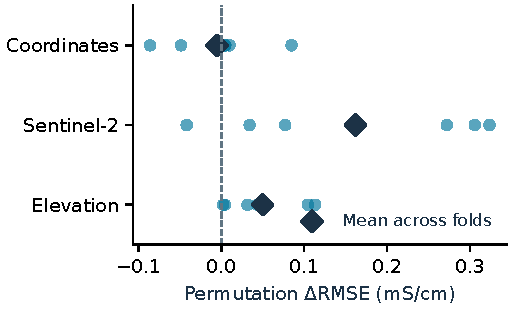
\includegraphics[width=\columnwidth]{permutation}
\caption{Change in held-out RMSE after shuffling predictor groups for Set E Auto. Circles show means over 20 repetitions for individual folds. Diamonds summarize the six fold means.}
\label{fig:importance}
\end{figure}

\section{Discussion}
The spatial design allows both years in training when sites are geographically eligible. The pooled scores can therefore benefit from broader response and predictor distributions than those available to a single-campaign model.

The all-predictor transfer results have $R^2$ close to zero in both directions, despite a smaller RMSE than tuned IDW in the reverse direction. A lower error against that comparator therefore gives limited evidence of practical transfer. In the spatial test, the large negative residuals at the high end suggest that a model with adequate pooled RMSE can still miss the most saline sites. Performance in that range matters if predictions are used to prioritize field sampling.

Surface reflectance and surface elevation provide observations at deployment sites, but both are imperfect proxies for the properties of a soil extract. Vegetation, irrigation, crop stage and tidal water exposure can change between image acquisition and sampling. The pre-collection rule prevents imagery recorded after the response from entering its feature vector. Seasonal composites with broader dates address different availability constraints. Reproducing the published Landsat benchmark would be valuable precisely because product and window choices are inseparable from validation and sampling differences in the currently available comparisons.

\section{Limitations and Threats to Validity}
Two years supply only two independent campaign units. The data do not cover a range of months within each year and the sites are not a repeated panel. Fold boundaries arise from one geometry and the 1 km buffer is a separation rule, rather than an estimate of the full spatial dependence range. The block bootstrap samples six observed regions and is especially uncertain for localized extremes. Neither the spatial nor transfer intervals are prediction intervals for a new individual point.

A single pixel can combine land covers and need not represent the soil sampling footprint. The optical mask may retain residual haze or exclude wet but informative surfaces. One pre-collection scene can yield a lag-dependent proxy. Elevation from a DSM is sensitive to above-ground objects and vertical error in flat terrain. We did not include rainfall, land cover, soil chemistry or hydrologic distances. Mapping or operational decisions in unobserved areas, seasons, or EC extremes require additional validation.

\section{Conclusion and Future Work}
\ConclusionText{} Repeated measurements at shared sites across months and years would strengthen the test of temporal transfer. Acquisition, evaluation code, predictions and figure source are available at \url{https://github.com/XDR-SAM/soil-salinity-ml-research}.

\section*{Acknowledgment}
We acknowledge Md.\ Mamun, Lecturer, Bangladesh University, for supervision. We thank the dataset creators for collecting, measuring and archiving the original field observations. Contains modified Copernicus Sentinel data (2024--2025). Produced using Copernicus WorldDEM-30 \textcopyright{} DLR e.V.\ 2010--2014 and \textcopyright{} Airbus Defence and Space GmbH 2014--2018 provided under COPERNICUS by the European Union and ESA, all rights reserved. EO data provided under COPERNICUS by the European Union and ESA.

\bibliographystyle{IEEEtran}
\bibliography{references}
\end{document}
